\newpage
\section{OOA-Klassenmodell}\label{ooa}\label{joern:ooa}
Im Folgenden wird unser auf Basis der Anforderungen unseres Planspiels
erstelltes Klassendiagramm der Analysephase aus \ref{OOA-Client} und
\ref{OOA-Server} auf \pageref{OOA-Client} und \pageref{OOA-Server} n�her
erl�utert. 

Das Klassendiagramm ist in zwei H�lften aufgeteilt. In dem ersten Teil werden
die Klassen f�r den Client und die Klassen, die f�r die r�ndliche Kommunikation
zwischen Server und Client genutzt werden, abgebildet. Der zweite Teil enth�lt
die Klassen des Servers und weitere Klassen und Interfaces, die f�r die
Kommunikation zwischen Server und Client vorgesehen sind.

Das Herzst�ck des Unternehmens, das auf Client-Seite vorgesehen ist, ist die
'Company' -Klasse. In ihr werden alle Entscheidungen des Spielers bearbeitet
und sie enth�lt alle Informationen, die der Spieler �ber sein Unternehmen
ben�tigt.
Dies sind die Mitarbeiter, die einzelnen Abteilungen und die Beziehungen, die zu
den einzelnen Regionen bestehen.

In den Beziehungen zu den Regionen werden entweder in einer 'ResourceRelation'
der Besitztum dieser Region erlangt und, sollte man schon eine solche Region
besitzen, auch die vorhandenen Geb�ude dieser Region gespeichert. Die
'CityRelation' enth�lt alle Informationen �ber die Bewohner einer Stadt und mit
dem 'Contract' auch �ber die Kunden des Unternehmens. Hier werden auch neue
Vertr�ge angeboten, um neue Kunden zu generieren.

Die Abteilungen des Unternehmens umfassen das 'Warehouse', das
'InvestmentManagement', den 'Research', die 'Finances' und das 'Marketing'. Im
Warehouse werden die Rohstoffe gelagert, die in Minen produziert werden und die
f�r die Produktion von Strom in den Kraftwerken ben�tigt werden.
Auch gehandelte Rohstoffe werden hier entnommen oder eingelagert.\\
Das InvestmentMangement beinhaltet alle Geb�ude (Minen und Kraftwerke) und
alle Grundst�cke (Regionen), die das Unternehmen besitzt. Hier werden neue Geb�ude
hinzugef�gt, Abschreibungen berechnet und Produktionsmengen, die sich aus einer
maximalen Produktion und dem Auslastungsfaktor berechnen, eingestellt und
ausgelesen.
Zudem besitzt jedes Kraftwerk mehrere 'PowerStationRelation', die beinhalten, 
wieviel Energie das Kraftwerk den einzelnen umliegenden St�dten
liefert. Diese Beziehung von einem Kraftwerk zu den St�dten ist vorgesehen,
damit die gewollte maximale Lieferentfernung von drei Feldern nicht
�berschritten wird.\\
Die Finances sind vorgesehen, um alle vier Quartale eine Bilanz und eine
Gewinn- und Verlustrechnung aufzustellen. Alle Einnahmen und Ausgaben werden
hier eingespeichert und aufbereitet.\\
Das Marketing ist vorgesehen, um die Beliebtheit und die Bekanntheit
bei den Kunden zu beeinflussen.\\
Der letzte Bereich, der Research, ist vorgesehen, um m�glicherweise eine aktive
Forschung einbauen zu k�nnen. Auf Grund von anderen Priorit�ten ist dieser aber 
nicht weiter modelliert und auch nicht in das entg�ltige Planspiel aufgenommen
worden.

Der Server erm�glicht es, das Spiel auf verschiedenen Rechnern zusammen �ber das
Netzwerk spielen zu k�nnen. Viele Entscheidungen des Spielers werden auf
Client-Seite berechnet und abgearbeitet. Lediglich die Entscheidungen und Daten,
die alle Spieler betreffen, wie zum Beispiel die vorgesehenden Energiepreise,
Gebote f�r eine Region und Energiekauf und -verkauf an der Energieb�rse, werden
direkt dem Server mitgeteilt. Auch bereits gebaute Geb�ude werden dem Server
mitgeteilt, so dass sie f�r jeden Spieler ersichtlich werden.

Die wichtigsten Ver�nderungen der anderen Spiele und das generelle Geschehen
in dem Spiel werden jedem Spieler bzw. Client mit einem generellen Update jede
Runde �bertragen. Hierzu wird jedem Client ein aktuelles 'Map'-Objekt
geschickt, aus dem nun alle wichtigen generellen Informationen entnommen werden
k�nnen. Lediglich die Kunden des Unternehmens sollen seperat in einem
'CityRelation'-Objekt �bertragen werden, wenn sich etwas an ihnen �ndert.

Die Verbindung zwischen Client und Server wird aufgebaut indem
sich der Client �ber die 'Client'-Klasse mit der 'Server'-Klasse auf Serverseite
verbindet. Dort wird die Verbindung akzeptiert und nach dem
'Thread-per-Connection'-Prinzip ein f�r jeden Clienten seperater Thread der
Klasse 'Connection' erstellt. Dieser empf�ngt alle Nachrichten der Clients und
gibt diese an die 'ServerGame'-Klasse weiter, die die Daten anschlie�end
verarbeitet und entsprechende �nderungen im Spiel, zumeist in dem Map-Objekt,
vornimmt.

\begin{figure}[H]
\centering
\hspace*{-30mm}
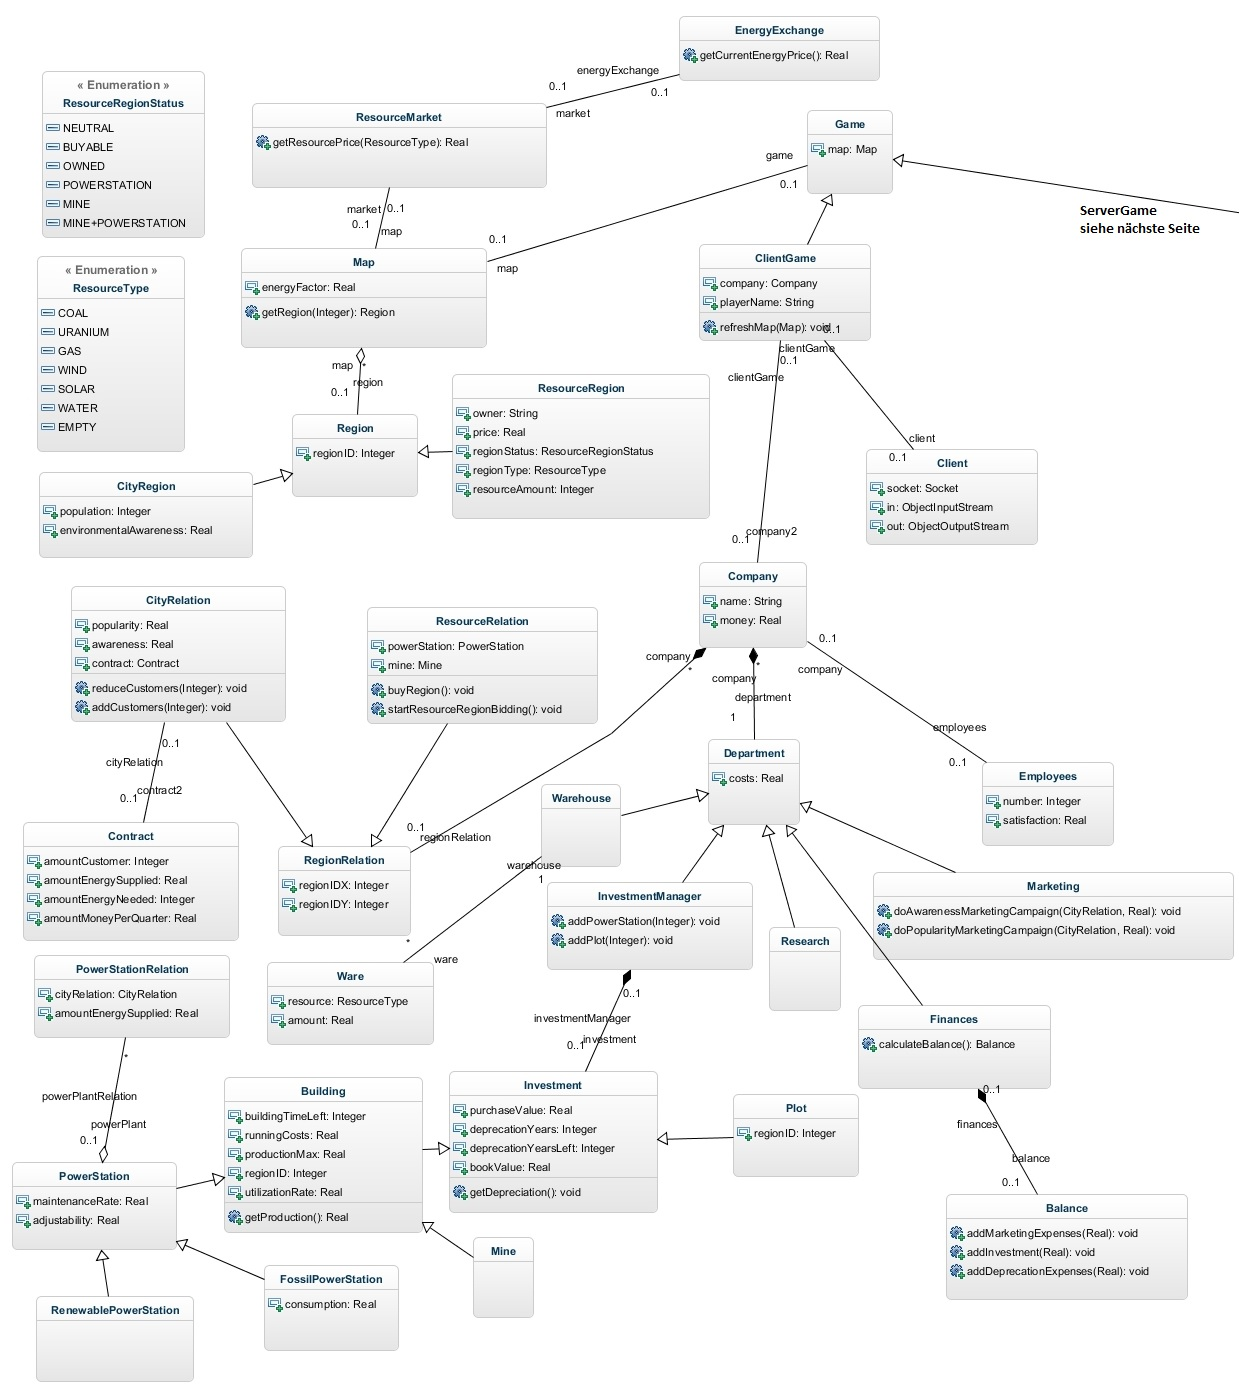
\includegraphics[width=1.3\textwidth]{se-wa-jpg/Client}
\caption{Klassendiagramm Teil 1}
\label{OOA-Client}
\end{figure}
%Die Grafik in Abbildung 
%\ref{labelname} auf Seite \pageref{labelname} ..
\begin{figure}[H]
\centering
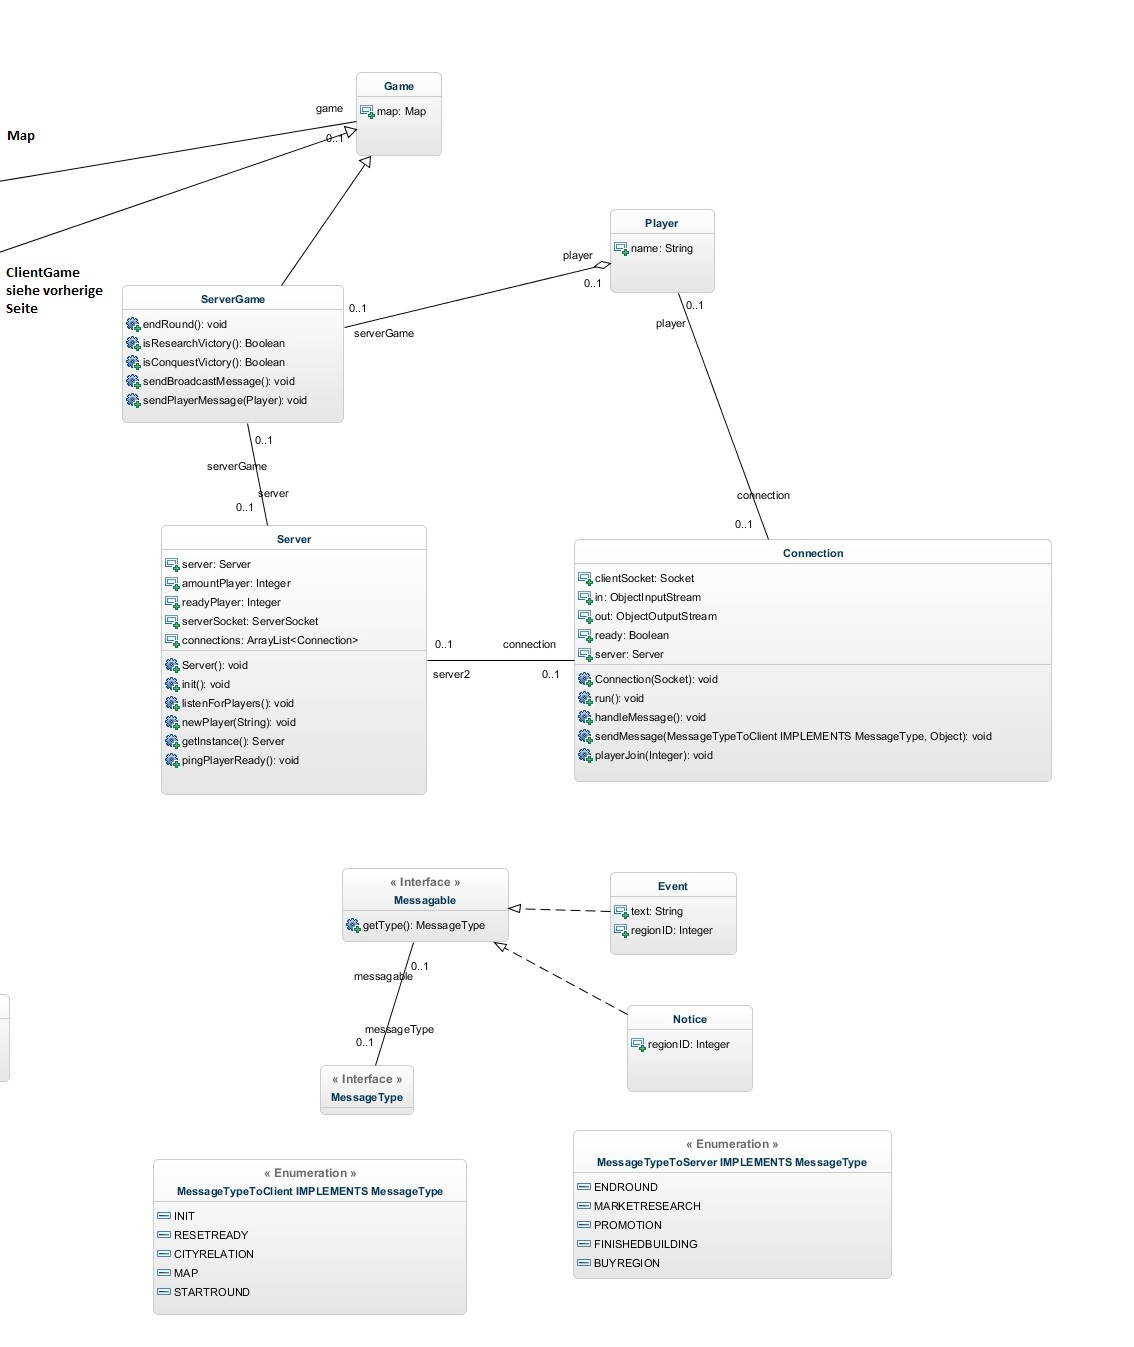
\includegraphics[width=1.1\textwidth]{se-wa-jpg/Server}
\caption{Klassendiagramm Teil 2}
\label{OOA-Server}
\end{figure}